\clearpage
\setcounter{page}{1}

\begin{center}
    \vspace*{3em}
    {\LARGE \textbf{Machine Exercise 7}}\\
    {\vspace{1.5em}}
    {\large Vending Machine}\\
\end{center}

\section{Introduction}
    For this machine exercise, you will implement a state machine using Verilog.
		
	\section{Vending Machine}
		\begin{enumerate}
			\item Implement a vending machine that sells one type of item: item A which costs PHP 2. Your top-level module should be defined as follows:
			
\begin{lstlisting}[style={verilog-style}, caption={Module declaration of the vending machine.} , label={code:vendo}]
module vendo(
	clk, nrst,
	sel_A,
	p_1, p_5,
	disp_A,
	change
);

	input clk, nrst;
	input sel_A;
	input p_1, p_5;
	output disp_A;
	output change;

endmodule
\end{lstlisting} 

			\item The general behavior of the vending machine should be as follows:
				\begin{enumerate}
					\item The \texttt{clk} and \texttt{nrst} inputs serve as the clock and active-low reset, respectively. Asserting \texttt{nrst} (setting it to 0) should set the outputs \texttt{disp\_A} and \texttt{change} to 0. Otherwise, the machine will go to the starting state of the vending process.
					
					\item From a starting state, the user selects the item to be dispensed. This is done using the \texttt{sel\_A} input. If item A (PHP 2) is selected, the user sets \texttt{sel\_A} to 1 for a clock cycle. The other inputs (\texttt{p\_1}, \texttt{p\_5}) are ignored during this step.
					
					\item After selecting the item, the user inputs coins using the \texttt{p\_1} and \texttt{p\_5} inputs. The \texttt{p\_1} and \texttt{p\_5} inputs represent PHP 1 and PHP 5 coins, respectively. For a single coin to be inserted, the corresponding input should be set to 1 for a clock cycle. We place a restriction that only one of the two inputs (\texttt{p\_1}, \texttt{p\_5}) can be set to 1 during this step of the vending process. This step repeats until there is enough money inserted for the selected item. The other input (\texttt{sel\_A}) is ignored during this step.
					
					\item Once enough money has been inserted, the machine immediately dispenses the item. If the user selected item A, \texttt{disp\_A} should be set to 1 on the same clock cycle that the last coin has been inserted. It is only during this step that the \texttt{disp\_A} output can be set to 1. Otherwise, it is set to 0 by default. All inputs (\texttt{sel\_A}, \texttt{p\_1}, \texttt{p\_5}) are ignored during this step. If the money inserted was exactly the same as the item cost, the machine then proceeds back to the starting state. Otherwise, the machine proceeds to dispense change.
					
					\item The machine dispenses change in PHP 1 increments. This is represented by the output \texttt{change}. The machine starts to dispense change in the same clock cycle that the item is dispensed. A single clock cycle where the output \texttt{change} is set to 1 represents a dispensed PHP 1 coin. This step is repeated until all change has been dispensed. It is only during this step that the output \texttt{change} can be set to 1. Otherwise, it is set to 0 by default. All inputs (\texttt{sel\_A} \texttt{p\_1}, \texttt{p\_5}) are ignored during this step. After dispensing all of the change, the machine then proceeds back to the starting state.
					
				\end{enumerate}
			
			\item Design a testbench that implements the timing diagram shown in Figure \ref{fig:testbench}. An example response of the machine is also included in the timing diagram below. Verify the functionality of your design (not yet synthesized) using this testbench. 
				\begin{figure}[!htbp]
					\centering
					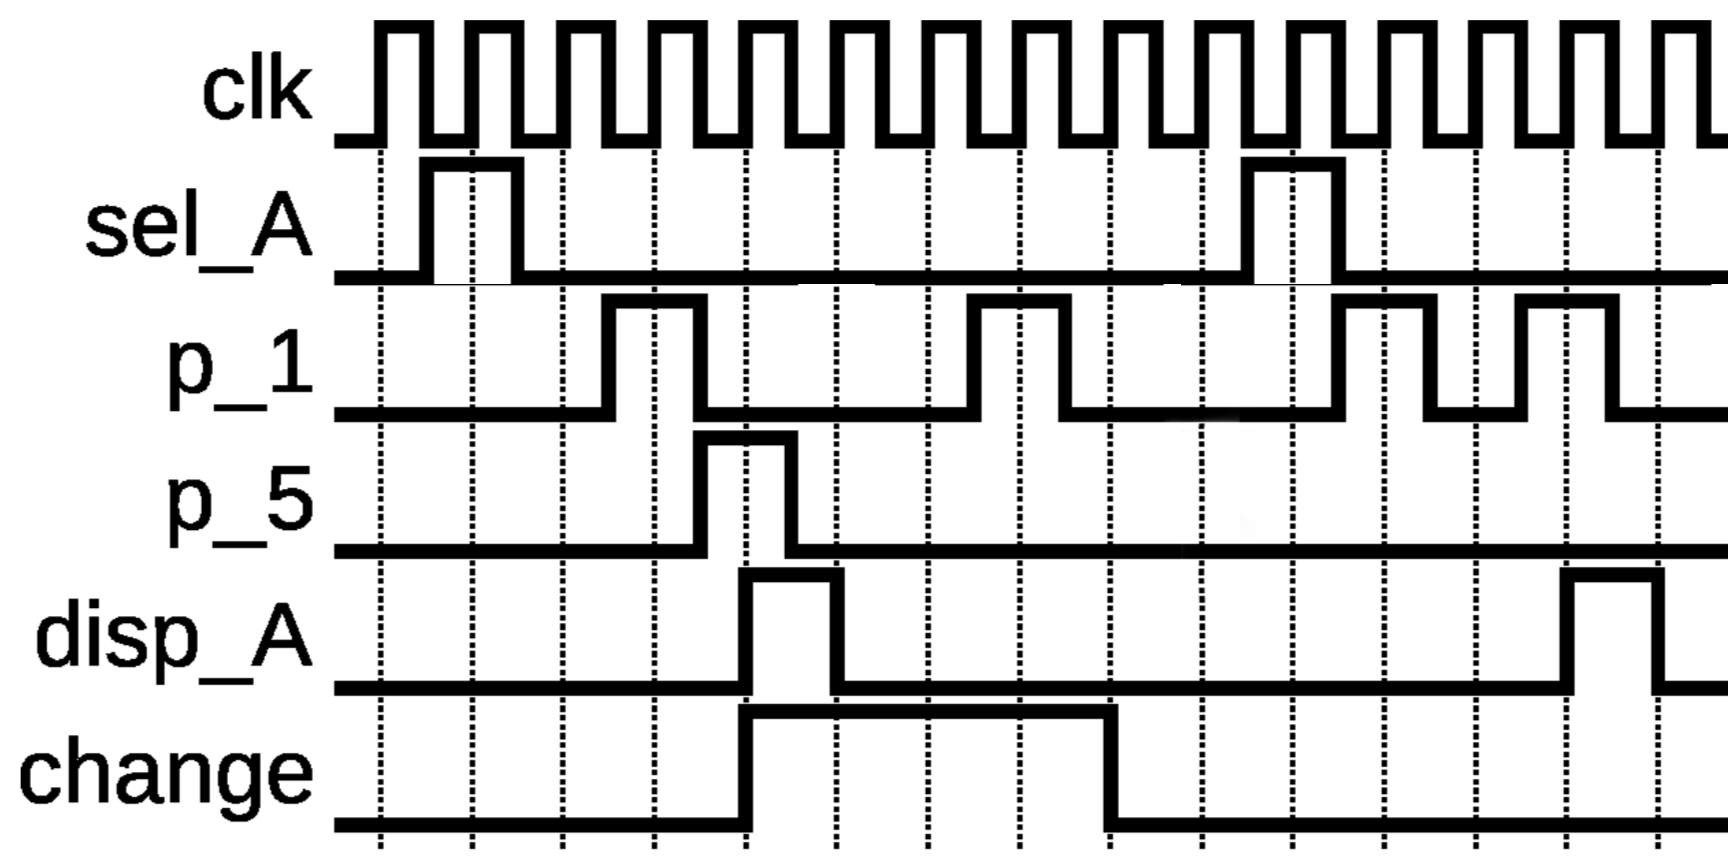
\includegraphics[width=0.55\textwidth]{me5_testbench}
					\caption{Vending machine testbench.}
					\label{fig:testbench}
				\end{figure}
			
			
			\item Implement your design on the Arty-7 35T Evaluation Kit board. Associate each port of your module to an FPGA pin as shown in the port mapping in Table \ref{tab:port}.
			
				\begin{table}[!htbp]
					\centering
					\caption{Port mapping.}
					\label{tab:port}
					\begin{tabular}{ | l | l | }
						\hline
						\multicolumn{1}{|c|}{Module Port} & \multicolumn{1}{c|}{FPGA Pin} \\
						\hline\hline
						\texttt{clk} & on-board $100MHz$ clock \\
						\hline
						\texttt{nrst} & SW0 \\
						\hline
						\texttt{sel\_A} BTN0 \\
						\hline
						\texttt{p\_1} & BTN1 \\
						\hline
						\texttt{p\_5} & BTN2 \\
						\hline
						\texttt{disp\_A} & LED1 \\
						\hline
						\texttt{change} & LED0 \\
						\hline
					\end{tabular}
				\end{table}
		\end{enumerate}